% Author: Rasmus Pank Roulund
\documentclass{standalone}
\usepackage{tikz}
\usetikzlibrary{shapes.geometric, arrows,positioning,calc,fit,patterns,intersections}
\usepackage{pgfplots}
\usepackage{relsize}
\usepackage{amssymb}

\newcommand*{\showinv}{}
\newcommand*{\showdiscr}{}
\newcommand*{\showfullobs}{}
\newcommand*{\showext}{}
\newcommand*{\showtransition}{}
\newcommand*{\showunobstrans}{}

\begin{document}

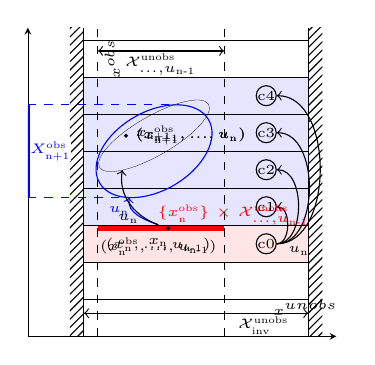
\begin{tikzpicture}

\pgfdeclarelayer{bg}    % declare background layer
\pgfsetlayers{bg,main}  % set the order of the layers (main is the standard layer)
\medmuskip=6mu plus 1mu minus 6mu\relax
%\setlength{\thickmuskip}{0mu}
%\setlength{\medmuskip}{0mu}

\tikzset{
    elli/.style args={#1:#2and#3}{
        draw,
        shape=ellipse,
        rotate=#1,
        minimum width=2*#2,
        minimum height=2*#3,
        outer sep=0pt,
    },
    /pgf/decoration/raise/.append code={
        \def\tikzdecorationsbrace{#1}
    },
    elli node/.style={
        circle,
        black,
        draw=none,
        midway,
        anchor=#1-90,
        inner sep=0pt,
        shift=(#1+90:\tikzdecorationsbrace+\pgfdecorationsegmentamplitude)
    }
}

\tikzstyle{cell} = [rectangle, minimum width=3cm, minimum height=1cm,text centered, draw=black, text width=3cm,on grid,auto]
\tikzstyle{ground}=[fill,pattern=north east lines,draw=none,minimum width=0.75cm,minimum height=0.3cm]



\begin{axis}[anchor=origin,
		    x label style={at={(axis description cs:0.9,0.15)},anchor=north},
		    y label style={at={(axis description cs:0.33,.9)},anchor=south},
			width=5.5cm,
			height=5.5cm,
			xlabel =\tiny  $x^{unobs}$,
  			ylabel =\tiny  $x^{obs}$,
		    xmin=-1.2,
		    xmax=1.0,
		    ymin=-1.0,
		    ymax=1.0,
		    xticklabels={,,},
		    yticklabels={,,},
		    axis line style= ultra thin,
		    ticks=none,
		    axis lines = left
		    ]
%% Draw invariant

\node[draw=none] (xn) at (axis cs:-0.2,-0.3) {};
\node[draw=none] (xnn) at (axis cs:-0.5,0.3) {};

\newcommand{\drawcell}[2]{
\coordinate (pt1) at ($(axis cs:-0.8,#1*0.24-1)$);
\coordinate (pt2) at ($(axis cs:0.8,#1*0.24-0.76)$);
\coordinate (#2) at ($(axis cs:0.5,#1*0.24-0.88)$);
\node[draw,circle,inner sep=0pt,minimum size=1pt] (n#2) at (#2) {\tiny #2};
}

\ifdefined\showdiscr
\drawcell{2}{c0}
\begin{pgfonlayer}{bg} \draw[draw=none,fill=red!10] (pt1) rectangle (pt2); \end{pgfonlayer}
\drawcell{3}{c1}
\begin{pgfonlayer}{bg} \draw[draw=none,fill=blue!10] (pt1) rectangle (pt2); \end{pgfonlayer}
\drawcell{4}{c2}
\begin{pgfonlayer}{bg} \draw[draw=none,fill=blue!10] (pt1) rectangle (pt2); \end{pgfonlayer}
\drawcell{5}{c3}
\begin{pgfonlayer}{bg} \draw[draw=none,fill=blue!10] (pt1) rectangle (pt2); \end{pgfonlayer}
\drawcell{6}{c4}
\begin{pgfonlayer}{bg} \draw[draw=none,fill=blue!10] (pt1) rectangle (pt2); \end{pgfonlayer}

\newcommand\anglea{0}
\newcommand\angleb{0}

\draw [->] (nc0) to [out=\anglea,in=\angleb] (nc1);
\draw [->] (nc0) to [out=\anglea,in=\angleb] (nc2);
\draw [->] (nc0) to [out=\anglea,in=\angleb] (nc3);
\draw [->] (nc0) to [out=\anglea,in=\angleb] node[anchor=north,pos=0.15,inner sep=4pt]{\tiny $u_{\scalebox{0.7}{n}}$} (nc4);
\fi

\ifdefined\showinv
\draw [ground] (axis cs:-0.9,-1) rectangle (axis cs:-0.8,1.0);
\addplot[mark=none,black] coordinates { (-0.8,-1) (-0.8,1) } ;
\draw [ground] (axis cs:0.9,1) rectangle (axis cs:0.8,-1.);
\addplot[mark=none,black] coordinates { (0.8,-1) (0.8,1) } ;
\fi

\ifdefined\showunobstrans

\addplot[mark=none,black,thin,dashed] coordinates { (0.2,-1) (0.2,1) } ;
\addplot[mark=none,black,thin,dashed] coordinates { (-0.7,-1) (-0.7,1) } ;

\draw[<->] (axis cs:-0.8,-0.85) --node[anchor=north,pos=0.8,inner sep =1pt] {\tiny $\mathcal{X}^{\scalebox{0.7}{unobs}}_{\scalebox{0.7}{inv}}$} (axis cs:0.8,-0.85); 

\draw[<->] (axis cs:-0.7,0.85) --node[anchor=north,pos=0.5,inner sep =1pt] {\tiny $\mathcal{X}^{\scalebox{0.7}{unobs}}_{...,u_{\scalebox{0.7}{n-1}}}$} (axis cs:0.2,0.85); 

\node[draw=none,anchor=south west,inner sep=1pt,xshift=-5pt,text=red] at (xn) {\tiny $\{ x_{\scalebox{0.7}{n}}^{\scalebox{0.7}{obs}} \} \times \mathcal{X}^{\scalebox{0.7}{unobs}}_{...,u_{\scalebox{0.7}{n-1}}}$}; 
\addplot[mark=none,red,ultra thick] coordinates { (-0.7,-0.3) (0.2,-0.3) } ;

\node[elli=-60:0.5cm and 0.8cm,fill=none,thin,blue] (ellunobs) at (axis cs:-0.3,0.2) {};

\draw [->,blue] (xn) to [out=160,in=-100] node[anchor=north east,pos=0.8,inner sep=0pt]{\tiny $u_{\scalebox{0.7}{n}}$} (ellunobs.south east);

\coordinate (ya)  at (axis cs:-1.2,1.);
\coordinate (or)  at (axis cs:-1.2,0);
\coordinate (pt1) at ($(or)!(ellunobs.south east)!(ya)$);
\draw [-,blue,dashed]  (pt1) -- (ellunobs.south east);
\coordinate (pt2) at ($(or)!(ellunobs.north west)!(ya)$);
\draw [-,blue,dashed]  (pt2) -- (ellunobs.north west);

\draw [-,blue,ultra thick]  (pt1) -- node[draw=none,fill=white,anchor=west,text=blue,inner sep = 0pt] {\tiny $X^{\scalebox{0.7}{obs}}_{\scalebox{0.7}{n+1}}$}(pt2);

\fi

\tikzstyle{stylexn}=[draw=none,anchor=north]
\tikzstyle{stylexnn}=[draw=none,anchor=west]
\coordinate (xnp) at (xn.west);
\coordinate (xnnp) at (xnn);

\ifdefined\showinv
\node[stylexn] (xnl) at (xnp) {\tiny $(x_{\scalebox{0.7}{n}}^{\scalebox{0.7}{obs}},...,u_{\scalebox{0.7}{n-1}})$};
\node[stylexnn] (xnnl) at (xnnp) {\tiny $(x_{\scalebox{0.7}{n+1}}^{\scalebox{0.7}{obs}},...,u_{\scalebox{0.7}{n}})$};
\fi

\ifdefined\showext
\node[stylexn] (xnl) at (xnp) {\tiny $(x_{\scalebox{0.7}{n}},...,u_{\scalebox{0.7}{n-1}})$};
\node[stylexnn] (xnnl) at (xnnp) {\tiny $(x_{\scalebox{0.7}{n+1}},...,u_{\scalebox{0.7}{n}})$};
\fi

\ifdefined\showfullobs
\node[stylexn] (xnl) at (xnp) {\tiny $x_{\scalebox{0.7}{n}}$};
\node[stylexnn] (xnnl) at (xnnp) {\tiny $x_{\scalebox{0.7}{n+1}}$};
\fi

\draw[mark=*,mark size=0.5,draw=none] plot coordinates {(xn)} -- plot coordinates {(xnn)} ;


\ifdefined\showtransition
\node[elli=-60:0.25cm and 0.8cm,fill=none,line width=0.1pt] (ell) at (axis cs:-0.3,0.3) {};

\draw [->] (xn) to [out=160,in=-100] node[anchor=north east,pos=0.3,inner sep=0pt]{\tiny $u_{\scalebox{0.7}{n}}$} (ell.south east);
\fi

\ifdefined\showdiscr
\begin{pgfonlayer}{bg}
\foreach \yindex in {-1,-0.76,...,1}
	\addplot[mark=none,black,ultra thin] coordinates { (-0.8,\yindex) (0.8,\yindex) } ;
\end{pgfonlayer}
\fi

\end{axis}

\end{tikzpicture}

\end{document}
